\chapter{Desarrollo y fases del producto}
A lo largo de esta sección comentaremos todo el proceso de desarrollo del prototipo y de la 
memoria, las diferentes iteraciones del producto serán agrupadas en diversas fases con el fin
de facilitar la lectura y el entendimiento de los objetivos planteados en cada momento. Además,
se contarán de forma más extensa los puntos relevantes y objetivos en este proyecto.

\section{Fase 0: Definición del proyecto y primeros pasos}

\begin{table}[htb]
\begin{center}
\begin{tabular}{|c|p{7cm}|c|c|}

\hline
Iteraciones & De la 0 a la 2                                                & Completado    & Terminado en \\ 
\hline
Objetivos   &   \textbf{0.1.} Definir la idea.                              & 60\%          & x         \\
		    &   \textbf{0.2.} Iniciar desarrollo del prototipo
		    					Integrar TinyPTC y dibujar por pantalla.    & 100\%         & x         \\
		    &	\textbf{0.3.} Adquirir hábito de escribir, preparar
		    					las herramientas y entorno de LaTex.        & 50\%          & x         \\
		    &	\textbf{0.4.} Prototipado del movimiento usando 
		    					\textit{Steering behavior}.                 & 30\%          & x         \\
	\cmidrule{2-2}
			&	\textbf{1.1.} Creación tipo con coma fija.                  & 100\%         & x         \\
		    &	\textbf{1.2.} Busqueda de referentes                        & 40\%          & x         \\
		    &	\textbf{1.3.} Corregir funcionamiento de los
		    					\textit{Steering behavior} y
		    					prototipar todos los posibles               & 100\%         & x         \\
		    &	\textbf{1.4.} Sistema de debug visual: vectores.            & 100\%         & x         \\ 
			&	\textbf{1.5.} Herramientras control de ejecución.           & 50\%          & x         \\ 
	\cmidrule{2-2}
		    &	\textbf{2.1.} Trabajar más la memoria.                      & 65\%          & x         \\
		    &	\textbf{2.2.} Terminar de definir idea (GDD).               & 100\%         & x         \\
		    &	\textbf{2.3.} Implementar el mínimo producto.               & 20\%          & x         \\
		    &	\textbf{2.4.} Experimentación y análisis de resultados.     & 0\%           & x         \\
\hline
\end{tabular}
\caption{Resumen fase 0}
\end{center}
\end{table}

\newpage

Esta primera fase engloba las tres primeras iteraciones donde comenzamos a terminar de definir 
la idea para el proyecto, ya que, todavía era un poco difusa la imagen del producto final que se
quería desarrollar.

Para ir entrando en una dinámica productiva iniciamos el desarrollo de funcionalidades básicas 
como pueden ser el bucle principal del juego, en el cual usamos de la librería \textit{\textless
chrono\textgreater} de C++ para medir y limitar el tiempo entre ejecuciones del bucle y el uso 
de una enumeración que contiene los posibles resultados de un ciclo del juego.

\begin{lstlisting}[style=CodigoC++, caption={Resultados iteración bucle},label=game_conditions]
enum class GameConditions : int16_t {
    Loop     = 0u, //continuar con el bucle
    Cerrar   = 1u, //terminar la ejecución del programa
    Derrota  = 2u, //el jugador a perdido
    Victoria = 3u  //el jugador a ganado
};
\end{lstlisting}

Una vez tenemos el bucle, toca introducir algo que hacer en el, como primer sistema del juego
encontramos el sistema de dibujado el cual se encargará de crear y manejar la ventana, además
de pintar nuestras entidades y herramientas visuales. Para incluir todas estas funcionalidades
sin añadir librerías pesadas incluiremos \textit{\textless TinyPTC\textgreater}, la cual no 
ncluye demasidas funcionalidades y opciones pero nos permitirá trabajar rápido y de forma 
sencilla. Los sprites en un inicio serán simples cuadrados de colores por lo que no requeriremos 
mucho.

Por último, se añadireron las componentes de movimiento y \ac{IA} que, junto a sus correspondientes
sistemas, nos permitirán poder crear un comportamiento de patrulla básico entre puntos fijos.
Además, se terminó la preparación de las herramientas de \LaTeX y `Jabref' para redactar la 
memoria acompañado de la lectura de las directrices, normas y memorias de compañeros del año 
pasado.

\begin{lstlisting}[style=CodigoC++, caption={Componente de Movimiento},label=mov_cmp]
struct MovementComponent : BECS::Component_t {

  explicit MovementComponent(const BECS::entID entityID, const fint_t<int64_t> c_X, const fint_t<int64_t> c_Y) 
    : Component_t(entityID), coords(c_X, c_Y) { }

  //posicion actual.
  fvec2<fint_t<int64_t>> coords           { { 0l }, { 0l } };
  //desplazamiento final de la entidad.
  fvec2<fint_t<int64_t>> dir              { { 0l }, { 0l } };
  //acceleracion hacia la posición deseada.
  fvec2<fint_t<int64_t>> accel_to_target  { { 0l }, { 0l } };
  //si hay entidades cercanas, fuerza que las agrupa.
  fvec2<fint_t<int64_t>> cohesion_force   { { 0l }, { 0l } };
  //si hay entidades cercanas, fuerza que las separa.
  fvec2<fint_t<int64_t>> separation_force { { 0l }, { 0l } };

  //aux debug mode
  fvec2<fint_t<int64_t>> sep_copy_to_draw { { 0l }, { 0l } };
  fvec2<fint_t<int64_t>> coh_copy_to_draw { { 0l }, { 0l } };
};
\end{lstlisting}

A lo largo de la iteración siguiente, seguimos añadiendo funcionalidades al prototipo como puede 
ser el componente y sistema de \textit{Input}, el cual nos permitirá interactuar con el juego
mediante el mapeado del teclado haciendo uso de la librería \textit{\textless X11\textgreater}
y \textit{\textless TinyPTC\textgreater}

Una de las herramientas implementadas en el proyecto es el tipo de dato entero con coma fija,
en C++ podemos encontrar el tipo fundamental \textit{float} creado para trabajar con números 
reales, pero si miramos como funcionan exactamente es posible encontar que no es lo que deseamos
exactamente. Los \textit{floats} usan ``precisión simple'' lo cual implica que conforme el número 
sea más grande, la cantidad de bytes destinados a la representación de la parte decimal va 
disminuyendo ofreciendo así menor precisión. Además, trabajar con ellos es más costoso a nivel
computacional\footnote{Esto pasa sobretodo en máquinas que no tengan CPUs con unidades destinadas 
a cálculos en coma flotante} y conllevan un código más pesado debido a la codificación usada 
al ser compilados.

El tipo con coma fija tiene dos partes, en primer lúgar el valor que se quiere reprentar normal
y corriente, y por otro la escala, número que indicará la cantidad de valores disponibles
para la representación decimal. La escala la usaremos para multiplicar o dividir nuestro número
para convertirlo a coma fija, devolverlo sin escalar y/o operaciones con otros números enteros.\\
Es importante elegir una escala adecuada para trabajar de forma eficiente, para ello escogeremos
un número portencia de 2 el cual nos permitirá usar desplazamientos en múltiplicaciones y divisiones,
hacíendo los calculos mucho más rápidos que si tuvieramos que usar las operaciones comunes.

\begin{lstlisting}[style=CodigoC++, caption={Entero coma fija},label=fint_t]
template <typename NumType>
struct fint_t {
    fint_t() = default;

    constexpr fint_t(NumType num)                noexcept; //ctor
    constexpr explicit fint_t(float   num)       noexcept; //ctor
    constexpr fint_t(const fint_t<NumType>& num) noexcept = default; 
    constexpr fint_t(fint_t<NumType>&& num)      noexcept = default;

/* OPERATIONS */
	//***

/* GETTERS */
    constexpr NumType getNoScaled() const noexcept;
    
/* DATA */    
                            NumType number { 0 };
    constexpr static inline NumType SCALE  { 65536 };
};
\end{lstlisting}


Por otro lado, se comenzó a trabajar en la \ac{IA} del juego creando los primeros comportamientos
y herramientas para alternar entre ellos. Aquí caeremos en los primeros errores de concepto a la
hora de trabajar con los \textit{`Steering behaviors'}, ya que, a la hora de implementar los
usamos un plateamiento y cálculos de movimiento cinético sin aceleración, trabajando directamente 
con la velocidad.\\
En su lugar, lo planteado por la técnica es usar la aceleración de la entidad, de esta forma se 
logrará calcular el movimiento deseado en un momento puntual, enfrentándo lo contra la velocidad 
acumulada. Esto nos proporcionará un movimiento continuado y dinámico en lugar de cambiar drásticamente de 
dirección y velocidad.

\begin{figure}[htb]
\centering
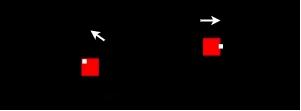
\includegraphics[width=0.35\textwidth]{imagenes/diario_desarrollo/mov1.png}
\caption{Movimiento rectilíneo uniforme.}
\label{fig:mru}
\end{figure} 

\begin{figure}[htb]
\centering
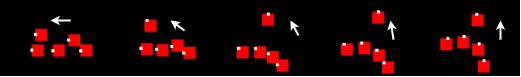
\includegraphics[width=1\textwidth]{imagenes/diario_desarrollo/mov2.png}
\caption{Movimiento rectilíneo acelerado.}
\label{fig:mra}
\end{figure} 

Uno de los comportamientos más sencillos es el \textit{`Arrive'}, el cual nos
llevará a la posición objetivo de forma directa y conforme estemos llegando a esta, la 
acceleración disminuirá parando una vez hayamos llegado al destino. En esta función podremos
apreciar como calculamos la velocidad objetivo en función de la distancia hasta llegar a
la posición objetivo, una vez se calcula se compara con el desplazamiento actual de la entidad
y es la resta de ambas la que nos dará la acceleración necesaria para alcanzar la velocidad
objetivo, siempre controlando que la acceleración y la velocidad no exceden los límites 
marcados.\\
Además, contamos con dos modeficadores adicionales como son el tiempo deseado para alcanzar el
objetivo y un límite de distancia con el objetivo para evitar solapes y/o oscilar sobre el.

\begin{lstlisting}[style=CodigoC++, caption={Arrive behavior}, label=ia_arrive] 
template <typename Context_t>
constexpr bool
AI_System<Context_t>::arrive(Context_t& context, BECS::entID eid) noexcept {
    /* Recogida de datos */

    //Las varaibles en mayúscula son constantes definidas fuera
    //los datos terminados en `2' usan distancia al cuadrado

    if(distance2 < ENT_ARRIVE_DIST2)
        return false;

    if(distance2 > ENT_SLOW_DIST2)
        target_speed = ENT_MAX_SPEED;
    else
        target_speed = ENT_MAX_SPEED * 
        		( target_dir.length_fix() / ENT_SLOW_DIST );
    
    target_dir.normalize();
    target_dir *= target_speed;

    my_accel  = (target_dir - my_direct);
    my_accel /= ENT_TIME_TO_TARGET;

    if(my_accel.length2() > ENT_MAX_ACCEL2) {
        my_accel.normalize();
        my_accel *= ENT_MAX_ACCEL;
    }

    return true;
}
\end{lstlisting}

Durante la tercera iteración nos centramos en la mejora de algunos \textit{`Steering behaviors'}
para terminar de hacerlos más fáciles de usar y combinar, con el fin de tener un código más 
limpio y legible, también se mejoró el uso de la coma fija añadiendo más operaciones y ajustando
el funcionamiento.

Por otro lado, se añadieron herramientas para debug del movimientos de las entidades y las
diferentes componentes de este, para el dibujado de los vectores se eligió el algoritmo de
`\citeauthor*{Bresenham1962}', ya que, nos permite dibujar las rectas de una forma efectiva
y sin consumir muchos recursos. Además, el algoritmo esta diseñado para trabajar con enteros,
cosa que hacemos a lo largo de todo el prototipo. En el esquema~\ref{fig:bresenham} la 
cuadricula blanca representa los pixeles de la plantalla, en color azul la recta ideal que
se busca dibujar y en amarillo la recta resultante del algoritmo.

\begin{figure}[ht]
\centering
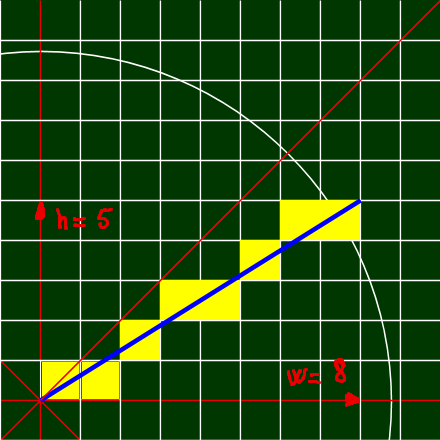
\includegraphics[width=0.35\textwidth]{imagenes/diario_desarrollo/linea_ideal.png}
\caption{Esquema algoritmo de Bresenham.}
\label{fig:bresenham}
\end{figure} 

Otra de las herramientas destinadas a poder análizar el funcionamiento del programa es
el control del tiempo de ejecución y el tamaño del \textit{`DeltaTime'}. Al poder disminuir
el número de fotogramas por segundo, podemos visualizar más detenidamente que sucede en
pantalla y ver que todo va según la previsión, por otra parte de puede aumentar la velocidad
para llegar antes a un punto de la ejecución en concreto. Además, jugar con el tamaño del
\textit{`DeltaTime'} nos permite experimentar con los valores de velocidad y/o otros factores
interpolados para ajustarlos de forma visual. 

Por último en cuanto a implementación, toda la información relacionada con el sistema de 
dibujado y los elementos visuales del juego se trabajan con \textit{uint64\_t}, mientras que
todo lo relacionado con el movimiento y demás calculos físicos se trabajan con
\textit{fint\_t\textless int64\_t\textgreater}. Por ello es necesario usar \textit{``casts``}
sobre los datos físicos con los que se quiera operar en el \textit{Render System}
\footnote{Ya sea la posición en el mapa como el sistema de debug para los vectores de
\textit{Steer}.}, como es una operación recurrente en el código se implementó un sistema 
auxiliar para convertir coordenada continuas (usadas en la mayoría de sistemas) a coordenadas de 
pantalla o pixel. 

\begin{figure}[ht]
\centering
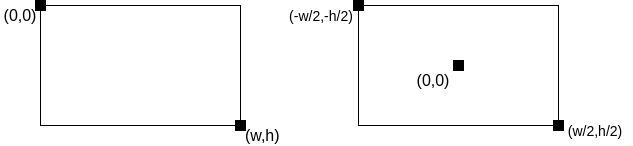
\includegraphics[width=0.8\textwidth]{imagenes/diario_desarrollo/sis_coords.png}\\
\hspace{-8mm} Coordenadas de pantalla. \hspace{16mm}  Coordenadas continuas.
\label{fig:sis_coords}
\end{figure} 

En lo referente a la memoria comenzamos la redacción de una versión preliminar del \ac{GDD}
donde comenzamos a describir las características del producto, del Estado del Arte donde se hace
mención a juegos que nos han servido de inspiración o modelo para imitar y se incluye una explicación
sobre las ténicas y algotimos se van a usar, y la explicación sobre la metodología seguida durante
este desarollo. 

\newpage

\section{Fase 1: Producto mínimo viable}

\begin{table}[ht]
\begin{center}
\begin{tabular}{|c|p{7cm}|c|c|}
\hline
Iteraciones & De la 3 a la 5                                               & \% Completado & Termindo en \\ 
\hline
Objetivos   &   \textbf{3.1.} Cambios en el motor ECS.                     & 100\% & x \\
		    &   \textbf{3.2.} Cambios en el almacenamiento de datos.       & 100\% & x \\ 
		    &	\textbf{3.3.} Cambio tipos propios a template.             & 100\% & x \\ 
		    &	\textbf{3.4.} Cambio en el sistema de clases.              & 100\% & x \\
	\cmidrule{2-2}
		    &	\textbf{4.1.} Añadir referente que use 
		    					\textit{Steering Behavior}.                & 100\% & x \\
		    &	\textbf{4.2.} Diagrama y explicación de las fases de 
		    					una iteración.                             & 100\% & x \\
            &   \textbf{4.3.} Agrupar iteración en fases y describir el
            					desarrollo hasta la fecha.                 & 20\%  & x \\
            &   \textbf{4.4.} Implementar mínimo producto.                 & 85\%  & x \\
            &   \textbf{4.5.} Análisis de resultados del MVP.              & 10\%  & x \\
	\cmidrule{2-2}
            &   \textbf{5.1.} Crear unidad de ataque a distancia.          & \% & x \\
		    &   \textbf{5.2.} Adición de formación en anillo.              & \% & x \\ 
		    &	\textbf{5.3.} Balanceo de las unidades.                    & \% & x \\ 
		    &	\textbf{5.4.} Profundizar los objetivos en el GDD y 
		    					explicar método de balanceo.               & \% & x \\ 
		    &	\textbf{5.5.} Incluir tabla resumen al inicio de fase
		    					e incluir información extra como el set-up.& \% & x \\
\hline
\end{tabular}
\caption{Resumen fase 1}
\end{center}
\end{table}

La fase comenzó con una iteración corta debido a las vacaciones de Navidad y final de año, en la
que el foco estuvo despositado en refactorizar y dejar en mejor estado el código desarrollado
hasta el momento, donde se separó el nucleo principal del motor \ac{ECS} del conjunto de sistemas y
herramientas en dos \textit{namespaces} diferentes. 

Por el lado del motor \ac{ECS}, en un primer lugar el almacén de componentes estaba diseñado
para contener punteros a componentes, esto implicaba que los datos de los componentes se
guardaban en la memoria libre de forma ``anárquica''~\ref{fig:memoria_ptr}, 
en su lugar, lo deseado es almacenar todas las componentes de forma contigua para poder utilizar
la caché cuando sea posible, para poder aprovechar que es más rápida y minimizar la cantidad de
veces que mandamos al sistema ir a buscar nuestros datos~\ref{fig:memoria_obj}.

\begin{figure}[htb]
\centering
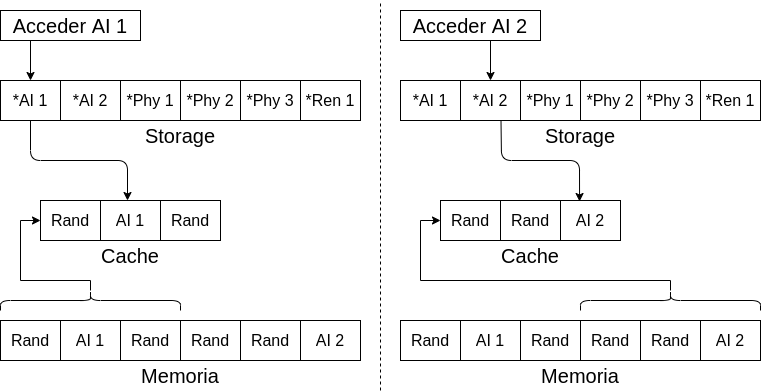
\includegraphics[width=0.7\textwidth]{imagenes/diario_desarrollo/memoria2.png}\\
\caption{Esquema acceso a vector de punteros.}
\label{fig:memoria_ptr}
\end{figure}

\begin{figure}[hbt]
\centering
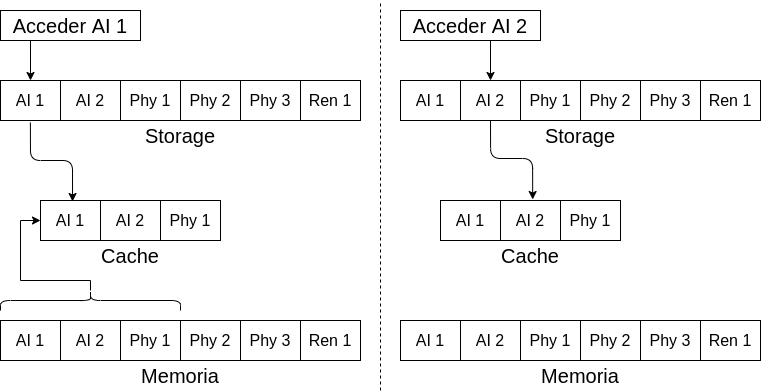
\includegraphics[width=0.7\textwidth]{imagenes/diario_desarrollo/memoria1.png}\\
\caption{Esquema acceso a vector de objetos.}
\label{fig:memoria_obj}
\end{figure}

%\placeholdertext{Comparativa tiempos/rendimiento a ser posible}

A continuación, se modificó la estructura de las entidades para componerse unicamente de su
\textit{Entity ID} y una serie de \textit{Component ID}s para posibles comprobaciones de que
componentes contiene la entidad, dejando así de tener un puntero a las entidades del almacén.
Esto implica una serie de cambios en la fachada y uso del \textit{Entity manager} a la hora
de crear/eliminar entidades y la obtención de las componentes desde los sistemas a través del
contexto. 

Por último se siguieron modificando los tipos propios, tanto el \textit{fint\_t} como
los \textit{vec2} y \textit{fvec2} para trabajar como plantillas, pudiendo así librarnos de
la necesidad de crear un tipo completo para cada tipo básico con el que queramos usarlos.

Durante el mes de enero se implementaron diversas funcionalidades, en primer lugar abordamos
el sistema de combate del juego, para ello se creó una componente para almacenar elementos como
la vida de la unidad, su daño, el rango y el tiempo entre ataques, además, los sistemas de 
ataque para ir restando vida a las unidades conforme reciban daño, el de \textit{cooldown} para
actualizar los temporizadores para volver a atacar, y por último el sistema de muertes donde se
manda a pedir que se borren las entidades que hayan muerto y se realizan las comprobaciones 
de victoria y derrota de la partida.

Una vez se resuelve la partida, en el bucle de ejecución del juego se reiniciarán el nivel
vaciando y volviendo a cargar los elementos del juego.

Para incluir los nuevos sistemas y funcionalidades a la rutina de las unidades, se ha ampliado
el apartado de toma de decisión incluyendo métodos para detectar si hay unidades enemigas 
cercanas y seleccionar como objetivo a la más cercana, que en caso de morir se lanzará una nueva
búsqueda. De forma similar, cuando no haya unidades enemigas cercanas se regresará al estado de
patrulla (en caso de la IA) y las manejadas por el jugador volveran a la posición de su
marcador en el mapa. 

En cuanto a las unidades de la partida, se creó un manejador de equipos donde se gestiona que
unidades pertenecen a cada facción, proporcionar métodos para obtener los \textit{ID}s de las
unidades por equipo e ir actualizando los equipos cuanda haya bajas. Además de, tener métodos
para crear tipos de unidades en concreto trabajando a la vez de ``fábrica''.

Por otro lado, en el apartado visual, se ha añadido un marcador que indica la dirección a la
que se esta orientando la entidad con el fin de dar \textit{feedback} al jugador y que se 
entienda mejor y de forma visual el desplazamiento o acción actual. Este marcador tiene un 
tamaño relativo al del sprite de la unidad y serán siempre de color blanco para que sea
fácil de identificar. 

\begin{figure}[h]
\centering
\begin{minipage}[c]{0.42\linewidth}
	\hspace{9mm}
	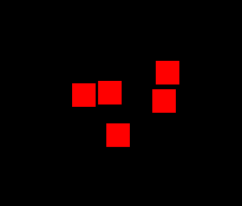
\includegraphics[width=0.7\textwidth]{imagenes/diario_desarrollo/sin-marcador.png} \\
	\label{sin_marcador}
\end{minipage}
\begin{minipage}[c]{0.40\linewidth}
	\hspace{9mm}
	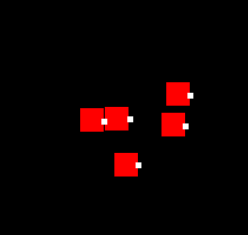
\includegraphics[width=0.7\textwidth]{imagenes/diario_desarrollo/marcador.png} \\
	\label{marcador}
\end{minipage} \\
	\hspace{0.5cm} Sin marcador. \hspace{3.5cm} Con marcador. 
\caption{Marcador dirección entidad.}
\end{figure}

Por último, en cuanto a la memoria, se ha añadido en el apartado de metodologia la
descripción de las fases que componen una iteración junto a un esquema. Se ha introducido
un tercer referente el cual basa toda su jugabilidad alrededor de los \textit{Steering
behavior}, debido a este juego hemos optado por cambiar la jugabilidad del proyecto
con el fin de imitar la de este juego y con intención de innovar en los controles, como ya se
refleja en el \ac{GDD}, actualmente el jugador no maneja directamente a las unidades con el
ratón ni las selecciona de forma individual, sino que controla un marcador verde el cual será
seguido por sus tropas y mediante ordenenes activará los distintos comportamientos de sus 
unidades. 



